% !TeX encoding = UTF-8
% !TeX spellcheck = fr_FR


\chapter{Cahier des charges}
\label{s:cdc}

Ce chapitre explique la procédure utilisée dans le but d'établir le cahier des charges.
Il expose les barèmes des différents objectifs.
De plus, le cahier des charges est synthétisé dans le tableau \ref{t:cdc_tab} et dans la maison de la qualité à la figure \ref{f:cdc_maison}.

% !TeX encoding = UTF-8
% !TeX spellcheck = fr_FR


\section{Automatisation}
\label{s:cdc_autonm}

Cette partie est essentielle à la réalisation de notre projet. \cite{parker1991mise}
En effet, l’automatisation lui permettra d’être autonome, fiable et précis lors de la prise de données.
Ainsi cette partie a une pondération de 20~\%.
% !TeX encoding = UTF-8
% !TeX spellcheck = fr_FR


\section{Communication}
\label{s:cdc_comm}

Deux barèmes constitueront l’évaluation de ce critère.
Premièrement, le système doit être facilement joignable et utilisable sans nécessiter une formation.

% !TeX encoding = UTF-8
% !TeX spellcheck = fr_FR


\subsection{Accès à distance}
\label{s:cdc_com_accadist}

Dans le but de rendre le système autonome et simplifier l’utilisation de celui-ci, une communication à distance doit être configurée.
Cette caractéristique est cruciale étant donné de la position du capteur, qui n’est pas facilement accessible, car il est placé à une certaine profondeur dans l’eau.
C’est pourquoi une pondération de 10~\% lui est associée. Deux éléments principaux constitueront l’évaluation de ce critère.
Premièrement, le système doit admettre une communication rapide à distance en tout temps.
Selon l’atteinte de ce critère, une valeur entre 0 et 1 leur sera transmise selon la réussite ou l’échec du critère.
La valeur est déterminé par la vitesse de la connexion selon cette formule où $x$ est la vitesse de connexion en $ko/s$:
\begin{equation} \label{eq:4.1.1}
	\ln \left( \frac{x-384}{6816} \right) +1,\qquad x \in [384,\,7200]
\end{equation}
% !TeX encoding = UTF-8
% !TeX spellcheck = fr_FR


\subsection{Facilité d’utilisation}
\label{s:cdc_com_faciutil}

Afin de rendre l’utilisation du système plus efficace et plus accessible, une interface facilement accessible doit être configurée pour assurer la communication à distance.
Un site web pourra assurer une facilité de connexion avec le système pour que n’importe quel opérateur du MFA puisse utiliser le système sans problèmes.
Ce critère aura une pondération de 5~\%.
Une interface simple et facilement utilisable obtiendra une note de 1, une interface complexe et qui provoque la confusion obtiendra la note de 0,5 et l’absence d’interface donnera la note de 0.
% !TeX encoding = UTF-8
% !TeX spellcheck = fr_FR


\section{Prise de données}
\label{s:cdc_prisdonn}

% !TeX encoding = UTF-8
% !TeX spellcheck = fr_FR


\subsection{Contrainte physique}
\label{s:cdc_pdd_cntphy}

Le client n’a pas indiqué de proportions claires à respecter pour la taille de notre système, celui-ci devra tout de même être le plus compact possible tout en assurant qu’une analyse sur un volume d’au moins un mètre cube d’eau soit possible.
Le système doit tolérer des températures entre 4~°C et 25~°C.
Afin d’éviter les problèmes de surchauffe, le produit final doit aussi compter un système de refroidissement automatique afin que la température intérieure soit au plus bas 10~°C en dessous de la température de l’eau et au plus haut cinq~°C au-dessus.
Le client demande aussi que le système soit assez résistant pour fonctionner à 15,25~m sous l’eau.
De plus, la limite de la masse de la partie submergée est fixée à 5 kilogrammes.
Un choix judicieux de matériaux légers, mais robustes est donc de mise.
Nous pondérons ce critère à 5~\%. Pour s’assurer de bien respecter ce critère, un tableau est fourni:

\begin{table}[htp]
	\caption{Barème de contraintes physiques}
	\label{tab:cdc_pdd_cntphy}
	\centering
	\begin{tabular}{|l|c|c|c|}
		\hline
		\multirow{2}{*}{\textbf{Partie évaluée}} & \multicolumn{3}{c|}{\textbf{Condition pour avoir la note de}} \\\cline{2-4}
		 & 0,2 & 0,15 & 0 \\\hline
		Volume analysé $V$ (m\textsuperscript{3}) & $V \ge 1$ & $V=1$ & $V<1$  \\\hline
		Température supportée $T$ (°C) & $4 \le T \le 25$  & non attribuée & 0 \\\hline
		Température par rapport à l'eau $\Delta T$ (°C) & $-10 \le \Delta T \le 5$ & non attribuée & 0 \\\hline
		Profondeur maximale $p$ (m) & $p \ge 15,25$ & $p=15,25$ & $p<15,25$    \\\hline
		Masse submergée $m$ (kg) & $m \ge 5$ & & $m < 5$  \\\hline
	\end{tabular}
\end{table}
% !TeX encoding = UTF-8
% !TeX spellcheck = fr_FR


\subsection{Capteur}
\label{s:cdc_pdd_capt}

Le client désire pouvoir récolter des données sur des spécimens d’au moins six centimètres.
Ainsi, il faut que la distance à laquelle la photo est prise résulte en une image d’au moins 16 pixels sur le capteur, ceux-ci étant le nombre maximal de pixels afin de pouvoir identifier quelque chose sur une photo.
Pour se faire, il faut que notre capteur produise une lumière suffisante à des distances maximales et minimales du volume d’analyse.
Il faut donc tenir compte de la relation inverse de la luminosité en fonction de la distance de la source.
Ce critère est important, car c’est celui qui assure la prise de photo qui est au cœur du projet. Ainsi on pondère ce critère à 5~\%.
Pour s’assurer du respect maximum de ce critère, la valeur de celui-ci est divisée en trois sous critères valant chacun 0,3 point, puis une fois que les valeurs seront additionnées, cela donnera un résultat sur 1.
% !TeX encoding = UTF-8
% !TeX spellcheck = fr_FR


\section{Sécurité}
\label{s:cdc_secu}

% !TeX encoding = UTF-8
% !TeX spellcheck = fr_FR


\subsection{Alarmes}
\label{s:cdc_sec_alar}

Selon la demande du client, le système sera composé d’un dispositif d’alarmes qui signalera l’opérateur dans le cas d’un problème.
Dans le cas d’un malfonctionnement ou d’un bris, une alarme sera levée à l’opérateur du MFA afin d’assurer une réparation rapide pour minimiser la période réfractaire.
Comme le système se trouve dans un milieu éloigné, il est important de savoir si le système fonctionne ou non.
C’est pourquoi une pondération de 5~\% sera affectée à ce critère.
Comme note, 1 sera attribué si les alarmes sont fonctionnelles et 0 si les alarmes sont absentes.
% !TeX encoding = UTF-8
% !TeX spellcheck = fr_FR


\subsection{Protection de l’accès à distance}
\label{s:cdc_sec_protaccdist}

Selon la demande du client, la transmission des informations et des alarmes doit être faite sur une connexion sécurisée avec le système en parallèle avec la communication à distance.
L’interception et le détournement des données pourraient avoir un impact nocif pour le fonctionnement du système (alarmes) et du logiciel de traitement (base de données).
Comme le système peut être dans un endroit éloigné comme dans un lac et difficilement détectable, il sera difficile pour un intrus de détecter le système et la connexion.
C’est pourquoi sa pondération sera de 4~\%.
L'équation \ref{eq:cdc_sec_protaccdist} calcule le barème, où $b$ est la longueur de la clé de chiffrement en bits.

\begin{equation}\label{eq:cdc_sec_protaccdist}
	\left(\frac{b-128}{960}\right)^2
\end{equation}
% !TeX encoding = UTF-8
% !TeX spellcheck = fr_FR


\subsection{Protection des données du client}
\label{s:cdc_sec_protdonnclnt}

Selon la demande du client, la base de données où seront enregistrées les données doit être sécurisée et confidentielle.
Il est important d’assurer ce critère, car toutes les images prises pour la détection doivent être stockées pendant une période d’au moins 2 ans selon la demande du client.
De plus, un intrus qui réussit à récupérer le système ne doit pas pouvoir accéder aux données, car la confidentialité de celles-ci sera compromise.
C’est pourquoi une pondération de 4~\% sera affectée à ce critère.
Comme note, 1 sera attribué si la sécurité de la base de données et la sécurité de l’accès physique au système est assurée, 0,5 si un seul de ces deux critères est assuré et 0 si elle n’est pas sécurisée.
% !TeX encoding = UTF-8
% !TeX spellcheck = fr_FR


\subsection{Protection de l’environnement}
\label{s:cdc_sec_protenv}

Comme la tâche qu’accomplit le système nécessite un écosystème aquatique en santé, il est important que celui-ci n’affecte pas l’environnement qu’il tente d’évaluer.
En cas de bris, le système doit être hermétique pour éviter les fuites dans le milieu.
Afin de protéger le système et les poissons qu’il évalue, il faudra accorder une attention particulière pour éviter que le système court-circuite avec l’eau et endommage l’écosystème.
C’est pourquoi une pondération de 2~\% sera affectée à ce critère.
Comme note, 1 sera attribué s’il n’y a aucun impact sur l’environnement et 0 s’il a un impact nocif sur l’écosystème.
% !TeX encoding = UTF-8
% !TeX spellcheck = fr_FR


\newpage

\begin{table}[htp]
	\caption{Tableau du cahier des charges}
	\label{t:cdc_tab}
	\centering
	\begin{tabular}{|l|c|c|c|c|}
		\hline\hline
		\textbf{\textit{Critères d’évaluation}} & \textbf{\textit{Pond. (\%)}} & \textbf{\textit{Barème}} & \textbf{\textit{Min}} & \textbf{\textit{Max}} \\
		\hline
		\hline
		\ref{s:cdc_autonm} \textbf{Automatisation} & \textbf{20} & & & \\
		\ref{s:cdc_aut_autnmi} Autonomie & 7 & Équation \ref{eq:cdc_aut_autnmi} & & \\
		\ref{s:cdc_aut_basedonn} Base de données & 3 & & & \\
		\ref{s:cdc_aut_config} Configurabilité & 7 & & 0 & 100 \\
		\ref{s:cdc_aut_fiabsys} Fiabilité du système & 3 & & & \\
		\hline
		\hline
		\ref{s:cdc_comm} \textbf{Communication} & \textbf{15} & & & \\
		\ref{s:cdc_com_accadist} Accès à distance & 10 & Équation \ref{eq:cdc_com_accadist} & & \\
		\ref{s:cdc_com_faciutil} Facilité d’utilisation & 5 & & & \\
		\hline
		\hline
		\ref{s:cdc_coutsech} \textbf{Coûts et échéances} & \textbf{15} & & & \\
		\ref{s:cdc_cee_coutproj} Coût du projet & 10 & Tableau \ref{tab:cdc_cee_coutproj} & & \\
		\ref{s:cdc_cee_rspech} Facilité d’utilisation & 5 & Tableau \ref{tab:cdc_cee_rspech} & & \\
		\hline
		\hline
		\ref{s:cdc_prisdonn} \textbf{Prise de données} & \textbf{10} & & & \\
		\ref{s:cdc_pdd_cntphy} Contrainte physique & 5 & Tableau \ref{tab:cdc_pdd_cntphy} & & \\
		\ref{s:cdc_pdd_capt} Capteur & 5 & & & \\
		\hline
		\hline
		\ref{s:cdc_secu} \textbf{Sécurité} & \textbf{15} & & & \\
		\ref{s:cdc_sec_alar} Alarmes & 5 & & & \\
		\ref{s:cdc_sec_protaccdist} Protection de l’accès à distance & 4 & & & \\
		\ref{s:cdc_sec_protdonnclnt} Protection des données du client & 4 & & & \\
		\ref{s:cdc_sec_protenv} Protection de l’environnement & 2 & & & \\
		\hline
		\hline
	\end{tabular}
\end{table}
% !TeX encoding = UTF-8
% !TeX spellcheck = fr_FR


\newpage

\begin{figure}[htp]
	\centering
	\caption{Maison de la qualité}
	\label{f:cdc_maison}
	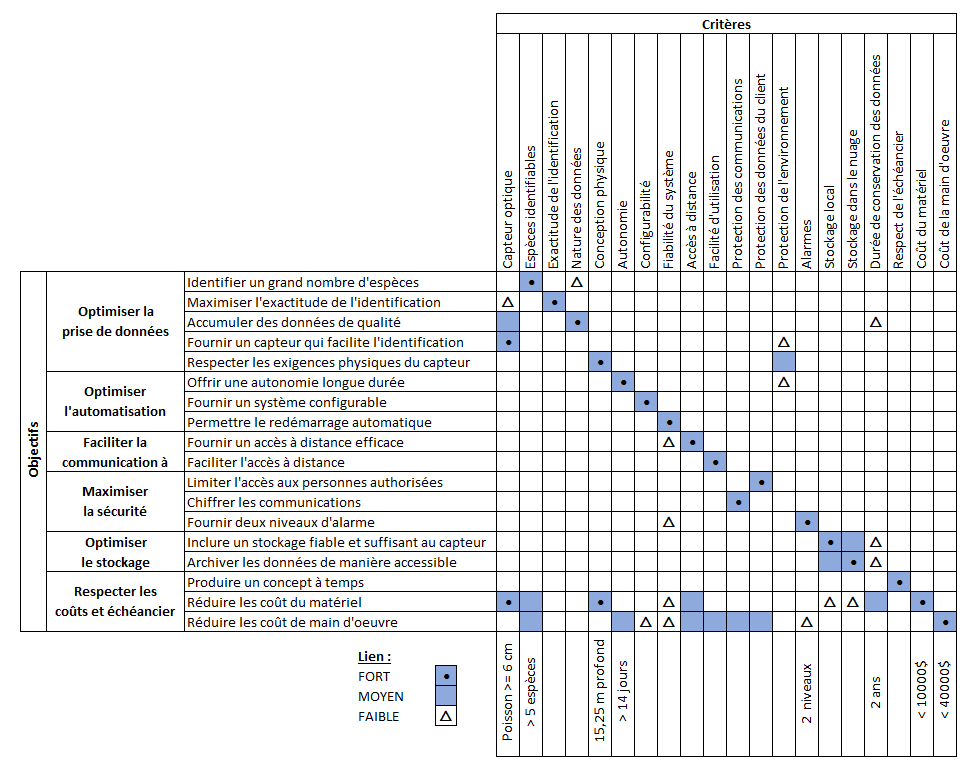
\includegraphics[width=\textwidth]{maison_qualite.png}
\end{figure}